\documentclass[border=3mm,
tikz,margin=2cm]{standalone}
\usetikzlibrary{arrows.meta,
calc, chains,
quotes,
positioning,
shapes.geometric}

\begin{document}
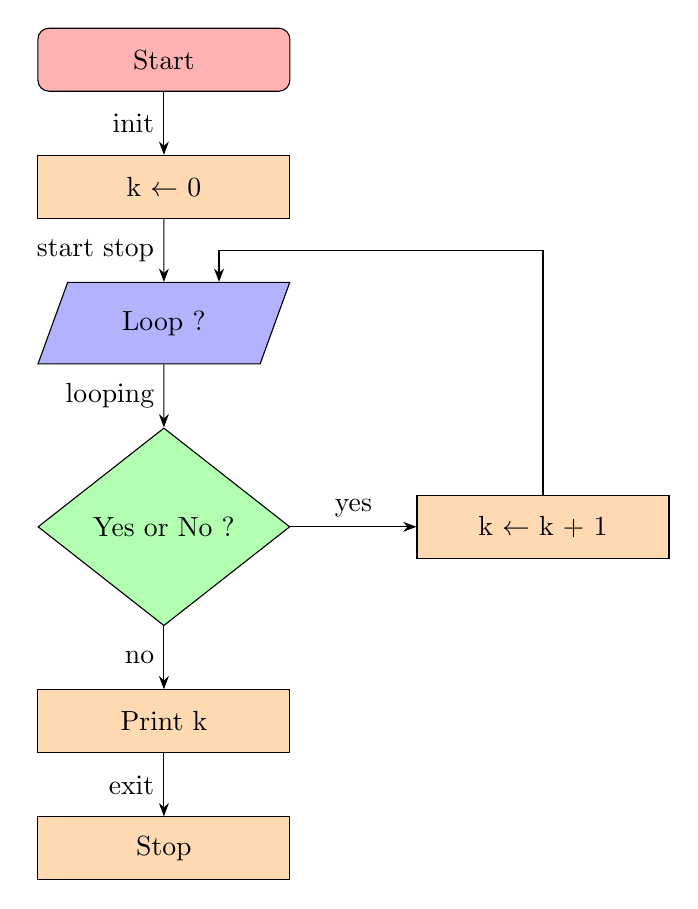
\begin{tikzpicture}[
    node distance = 8mm and 16mm,
        start chain = A going below,
        base/.style = {draw, minimum width=32mm, minimum height=8mm,
                       align=center, on chain=A},
        startstop/.style = {base, rectangle, rounded corners, fill=red!30},
        process/.style = {base, rectangle, fill=orange!30},
        io/.style = {base, trapezium, 
        trapezium left angle=70, trapezium right angle=110,
        fill=blue!30},
        decision/.style = {base, diamond, fill=green!30},
        every edge quotes/.style = {auto=right}
        ]

    \node [startstop]       {Start};            % <-- A-1
    \node [process]         {k $\leftarrow$ 0};
    \node [io]              {Loop ?};
    \node [decision]        {Yes or No ?};
    \node [process]         {Print k};
    \node [process]         {Stop};             % <-- A-6
    %
    \node [process,                             % <-- A-7
           right=of A-4]    {k $\leftarrow$ k + 1};
    %%
    \draw [arrows=-Stealth] 
        (A-1) edge["init"]          (A-2)
        (A-2) edge["start stop"]    (A-3)
        (A-3) edge["looping"]       (A-4)
        (A-4) edge["no"]            (A-5)
        (A-5) edge["exit"]          (A-6)
        (A-4) edge["yes"']          (A-7)       % <-- by ' is swapped label position
        (A-7) |- ($(A-2.south east)!0.5!(A-3.north east)$)
              -| ([xshift=7mm] A-3.north)
            ;
\end{tikzpicture}
\end{document}